\documentclass[10pt,a4paper]{article}
\usepackage[margin=1.5cm,top=1.4cm,bottom=1.6cm]{geometry}
\usepackage{fontspec}
% Police : EB Garamond, comme le roman (TeX Live : paquet ebgaramond ; Arch : texlive-fontsextra).
\IfFontExistsTF{EB Garamond}{\setmainfont{EB Garamond}[Ligatures=TeX]}%
  {\setmainfont{EBGaramond}[Extension=.otf, UprightFont=*-Regular, ItalicFont=*-Italic, BoldFont=*-SemiBold, BoldItalicFont=*-SemiBoldItalic, Ligatures=TeX]}
\newcommand{\caps}[1]{{\addfontfeature{LetterSpace=8}\fontsize{0.82em}{1em}\selectfont\MakeUppercase{#1}}}
\usepackage{xcolor}
\usepackage{tikz}
\usetikzlibrary{patterns}
\usepackage{enumitem}
\usepackage{microtype}
\frenchspacing
\setlength{\parindent}{0pt}\setlength{\parskip}{4pt}
\definecolor{wallc}{HTML}{2B2A33}
\definecolor{cRec}{HTML}{F1DDB8}
\definecolor{cFam}{HTML}{D6E4D9}
\definecolor{cSrv}{HTML}{DADBDF}
\definecolor{cCir}{HTML}{FAF8F3}
\definecolor{cExt}{HTML}{E7EEF3}
\definecolor{cSan}{HTML}{D9E3EF}
\definecolor{cGarden}{HTML}{CFE2C4}
\definecolor{accent}{HTML}{8A5A1F}
\tikzset{
  rec/.style={fill=cRec}, fam/.style={fill=cFam}, srv/.style={fill=cSrv}, cir/.style={fill=cCir},
  ext/.style={fill=cExt}, san/.style={fill=cSan}, garden/.style={fill=cGarden},
  road/.style={fill=cSrv!70}, pave/.style={fill=cSrv!40}, earth/.style={fill=accent!25},
  wall/.style={draw=wallc, line width=0.7pt}, extwall/.style={draw=wallc!60, line width=0.4pt, dashed},
  outer/.style={draw=wallc, line width=1.6pt},
  tread/.style={draw=wallc!55, line width=0.3pt}, stair/.style={draw=wallc, line width=0.4pt, fill=cCir},
  jamb/.style={draw=wallc, line width=0.5pt}, fold/.style={draw=wallc, line width=0.5pt, dash pattern=on 1.2pt off 1.2pt},
  lab/.style={font=\fontsize{6.2}{7.2}\selectfont, align=center, inner sep=0pt},
  tiny/.style={font=\fontsize{5.6}{6.4}\selectfont, inner sep=0.5pt},
  numtag/.style={font=\fontsize{5.6}{6.4}\selectfont\bfseries, fill=white, inner sep=0.8pt, rounded corners=0.6pt},
}
\newlist{descr}{description}{1}
\setlist[descr]{font=\normalfont, leftmargin=2.2em, labelwidth=1.9em, labelsep=0.3em, itemsep=2.5pt, parsep=0pt, topsep=2pt}
\newcommand{\legende}{%
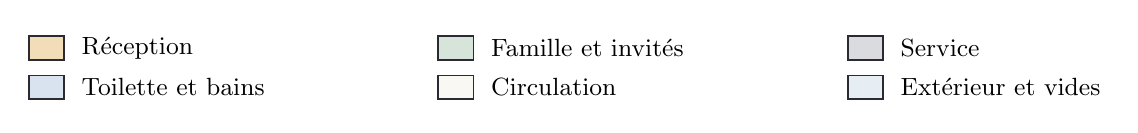
\begin{tikzpicture}[x=1cm,y=1cm]
\foreach \c/\t [count=\i from 0] in {rec/Réception, fam/Famille et invités, srv/Service, san/Toilette et bains, cir/Circulation, ext/Extérieur et vides}{
  \fill[\c] ({mod(\i,3)*5.2},{-int(\i/3)*0.5}) rectangle +(0.45,0.3); \draw[wall] ({mod(\i,3)*5.2},{-int(\i/3)*0.5}) rectangle +(0.45,0.3);
  \node[anchor=west,font=\small] at ({mod(\i,3)*5.2+0.55},{-int(\i/3)*0.5+0.15}) {\t};
}
\end{tikzpicture}}
\newcommand{\niveau}[1]{\par\noindent{\color{accent}\fontsize{17}{20}\selectfont\itshape #1}\par\vspace{2pt}}
\begin{document}

{\color{accent}\fontsize{26}{30}\selectfont\itshape La maison Whitmore}\par
{\large Belgravia, Londres — plans de travail, novembre 1890}\par\vspace{6pt}
Grande maison de ville mitoyenne d'un \emph{terrace} de Belgravia, en stuc blanc. Le plan suit le modèle d'une bonne maison londonienne publié par Robert Kerr dans \emph{The Gentleman's House} (3\textsuperscript{e} éd., 1871, pl.~XLII), un peu élargi : 36~ft de façade (11~m) au lieu de 32~ft~½, que Kerr tient pour le minimum d'une « really good house ». La parcelle fait environ 146~ft de profondeur (44,5~m), écuries comprises.

\textbf{Principes d'organisation.} Deux escaliers desservent la maison : le grand escalier pour la famille et les invités, l'escalier de service et son monte-charge pour les domestiques, du sous-sol aux combles. Les pièces de réception sont au rez-de-chaussée et au premier étage, les chambres au-dessus, les domestiques en bas et sous les toits. Éclairage au gaz, cheminées à charbon dans toutes les pièces, salles de bain à eau chaude : une maison riche et moderne de 1890.

\textbf{Conventions.} Unités en pieds anglais (1~ft $\approx$ 0,305~m). Sur chaque plan, la rue est en bas et le jardin en haut. Les cotes sont indicatives : elles servent à garder des volumes cohérents, pas à construire. Les descriptions restent générales et seront affinées scène par scène.

\vspace{4pt}\legende\par\vspace{8pt}


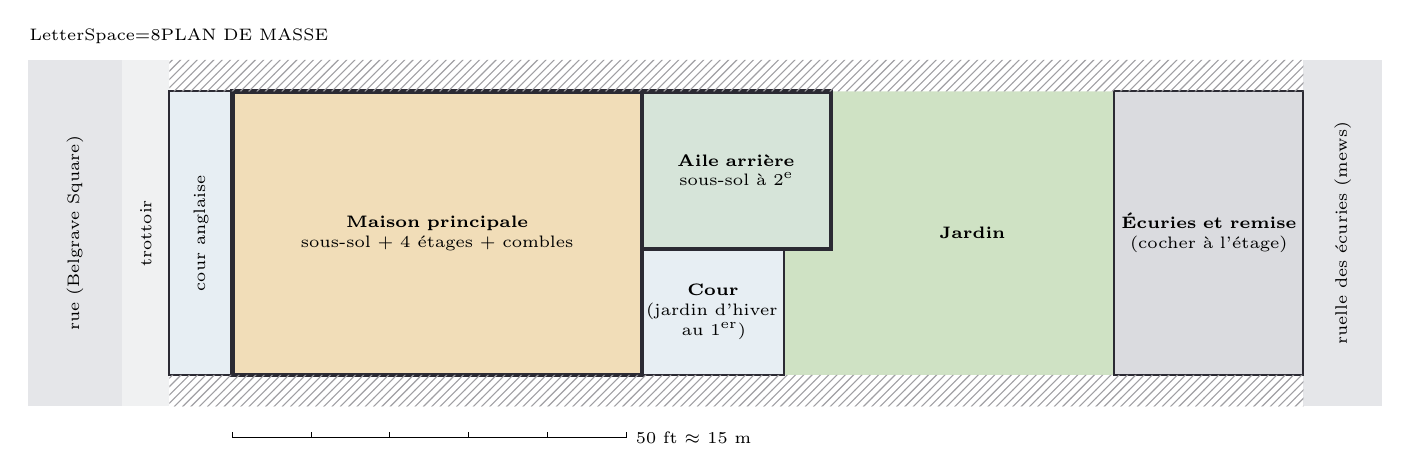
\begin{tikzpicture}[x=0.1cm,y=0.1cm]
% profondeur -> x ; largeur -> y
\fill[road] (-26,-4) rectangle (-14,40);
\node[tiny,rotate=90] at (-20,18) {rue (Belgrave Square)};
\fill[pave] (-14,-4) rectangle (-8,40);
\node[tiny,rotate=90] at (-11,18) {trottoir};
\fill[ext] (-8,0) rectangle (0,36);
\fill[rec] (0,0) rectangle (52,36);
\fill[fam] (52,16) rectangle (76,36);
\fill[ext] (52,0) rectangle (70,16);
\fill[garden] (70,0) rectangle (112,16) (76,16) rectangle (112,36);
\fill[srv] (112,0) rectangle (136,36);
\fill[road] (136,-4) rectangle (146,40);
\draw[outer] (0,0) rectangle (52,36);
\draw[outer] (52,36) -- (76,36) -- (76,16) -- (52,16);
\draw[wall] (-8,0) rectangle (0,36) (52,0) rectangle (70,16) (112,0) rectangle (136,36);
\fill[pattern=north east lines, pattern color=wallc!45] (-8,-4) rectangle (136,0) (-8,36) rectangle (136,40);
\node[tiny] at (-4,18) [rotate=90] {cour anglaise};
\node[lab, text width=4.4cm] at (26,18) {\textbf{Maison principale}\\ sous-sol + 4 étages + combles};
\node[lab, text width=2.2cm] at (64,26) {\textbf{Aile arrière}\\ sous-sol à 2\textsuperscript{e}};
\node[lab, text width=1.7cm] at (61,8) {\textbf{Cour}\\ (jardin d'hiver au 1\textsuperscript{er})};
\node[lab, text width=3.5cm] at (94,18) {\textbf{Jardin}};
\node[lab, text width=2.3cm] at (124,18) {\textbf{Écuries et remise}\\ (cocher à l'étage)};
\node[tiny,rotate=90] at (141,18) {ruelle des écuries (mews)};
% échelle
\draw[thin] (0,-8) -- (50,-8); \foreach \i in {0,10,...,50} \draw[thin] (\i,-8) -- (\i,-7.2);
\node[tiny,anchor=west] at (51,-8) {50 ft $\approx$ 15 m};
\node[tiny,anchor=west] at (-26,43) {\caps{plan de masse}};
\end{tikzpicture}

\par\vspace{10pt}

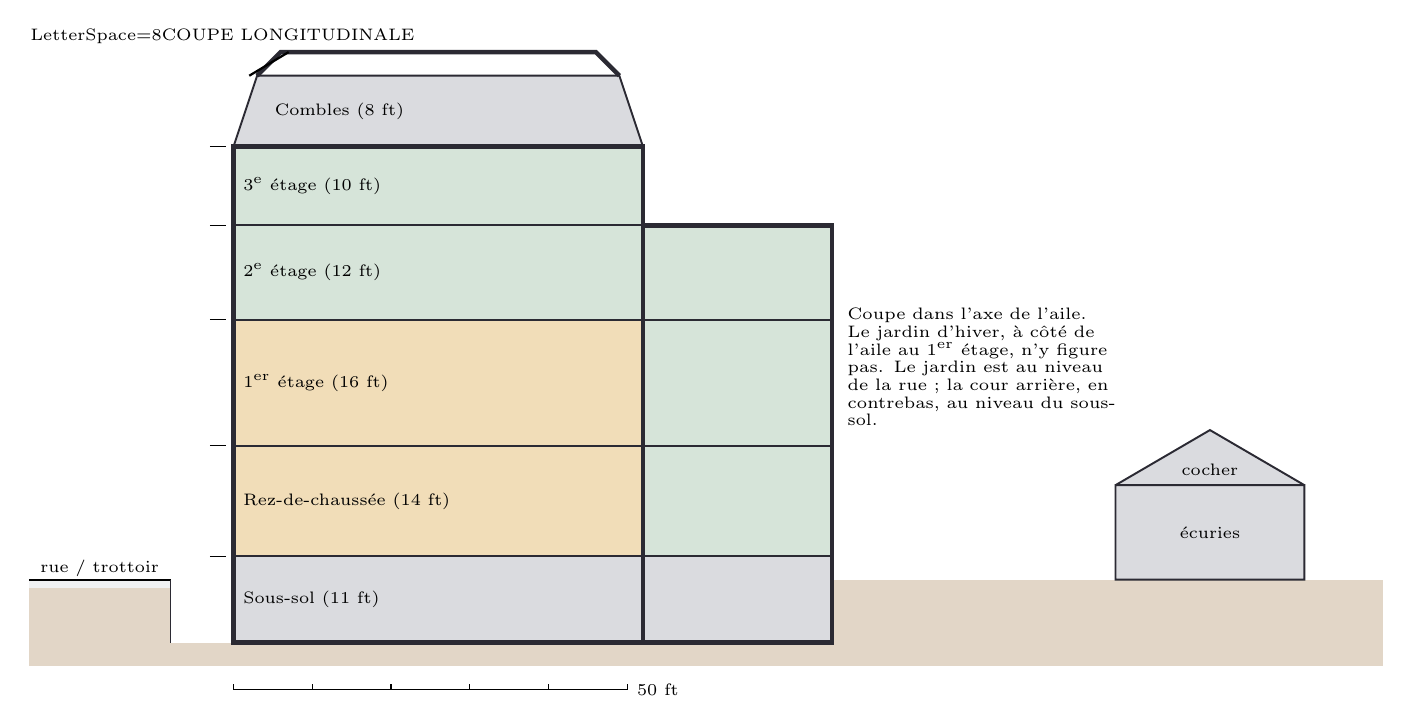
\begin{tikzpicture}[x=0.1cm,y=0.1cm]
% coupe longitudinale : x = profondeur (ft), y = hauteur (ft), rue a y = -3
\fill[pave] (-26,-3) rectangle (-8,-4);
\draw[thick] (-26,-3) -- (-8,-3);
\node[tiny] at (-17,-1.6) {rue / trottoir};
% sol
\fill[earth] (-8,-14) rectangle (146,-11);
\fill[earth] (-26,-14) rectangle (-8,-4);
\fill[earth] (76,-11) rectangle (146,-3);
% cour anglaise
\draw[wall] (-8,-11) -- (-8,-3);
% niveaux maison principale
\foreach \a/\b/\c/\n in {-11/0/srv/Sous-sol (11 ft), 0/14/rec/Rez-de-chaussée (14 ft), 14/30/rec/1\textsuperscript{er} étage (16 ft), 30/42/fam/2\textsuperscript{e} étage (12 ft), 42/52/fam/3\textsuperscript{e} étage (10 ft)} {
  \fill[\c] (0,\a) rectangle (52,\b);
  \draw[wall] (0,\a) rectangle (52,\b);
  \node[tiny,anchor=west] at (1,{(\a+\b)/2}) {\n};
}
% combles mansardés
\fill[srv] (0,52) -- (3,61) -- (49,61) -- (52,52) -- cycle;
\draw[wall] (0,52) -- (3,61) -- (49,61) -- (52,52);
\draw[outer] (3,61) -- (6,64) -- (46,64) -- (49,61);
\node[tiny,anchor=west] at (5,56.5) {Combles (8 ft)};
% aile
\foreach \a/\b/\c in {-11/0/srv, 0/14/fam, 14/30/fam, 30/42/fam} { \fill[\c] (52,\a) rectangle (76,\b); \draw[wall] (52,\a) rectangle (76,\b); }
% écuries
\fill[srv] (112,-3) rectangle (136,9); \fill[srv] (112,9) -- (124,16) -- (136,9) -- cycle;
\draw[wall] (112,-3) rectangle (136,9) (112,9) -- (124,16) -- (136,9);
\node[tiny] at (124,3) {écuries};
\node[tiny] at (124,11) {cocher};
\draw[outer] (0,-11) rectangle (52,52);
\draw[outer] (52,-11) rectangle (76,42);
% verrière
\draw[thick] (2,61) -- (7,64);
% repères de hauteur
\foreach \h in {0,14,30,42,52} \draw[thin] (-3,\h) -- (-1,\h);
\node[tiny,anchor=west] at (-26,66) {\caps{coupe longitudinale}};
\node[tiny,text width=3.4cm,align=left] at (95,24) {Coupe dans l'axe de l'aile. Le jardin d'hiver, à côté de l'aile au 1\textsuperscript{er} étage, n'y figure pas. Le jardin est au niveau de la rue ; la cour arrière, en contrebas, au niveau du sous-sol.};
\draw[thin] (0,-17) -- (50,-17); \foreach \i in {0,10,...,50} \draw[thin] (\i,-17) -- (\i,-16.2);
\node[tiny,anchor=west] at (51,-17) {50 ft};
\end{tikzpicture}

\par\vspace{6pt}
\textbf{Hauteurs sous plafond (ordres de grandeur).} Sous-sol 11~ft (3,35~m) ; rez-de-chaussée 14~ft (4,25~m) ; premier étage 16~ft (4,90~m), le plus haut, car c'est l'étage de réception ; deuxième 12~ft (3,65~m) ; troisième 10~ft (3,05~m) ; combles 8~ft (2,45~m). Le rez-de-chaussée est surélevé de quelques marches par rapport à la rue ; le sous-sol est à demi enterré.

\newpage
\niveau{Sous-sol — les offices}
{\small\textit{Hauteur : env. 11 ft sous plafond (3,35 m) ; à demi enterré, éclairé par la cour anglaise côté rue et par la cour arrière côté jardin.}}\par
{\small Le domaine des domestiques. On y accède depuis la rue par l'escalier de la cour anglaise (fournisseurs, domestiques), jamais par la porte d'entrée. Kerr place ici toute la vie de service : « Kitchen, Scullery, Pantry, and Larder; Butler's Pantry, Bedroom, Safe […] Housekeeper's-room, Still-room, Store-room, and Servants'-Hall ».}\par\vspace{4pt}
\noindent\begin{minipage}[t]{8.75cm}\vspace{0pt}
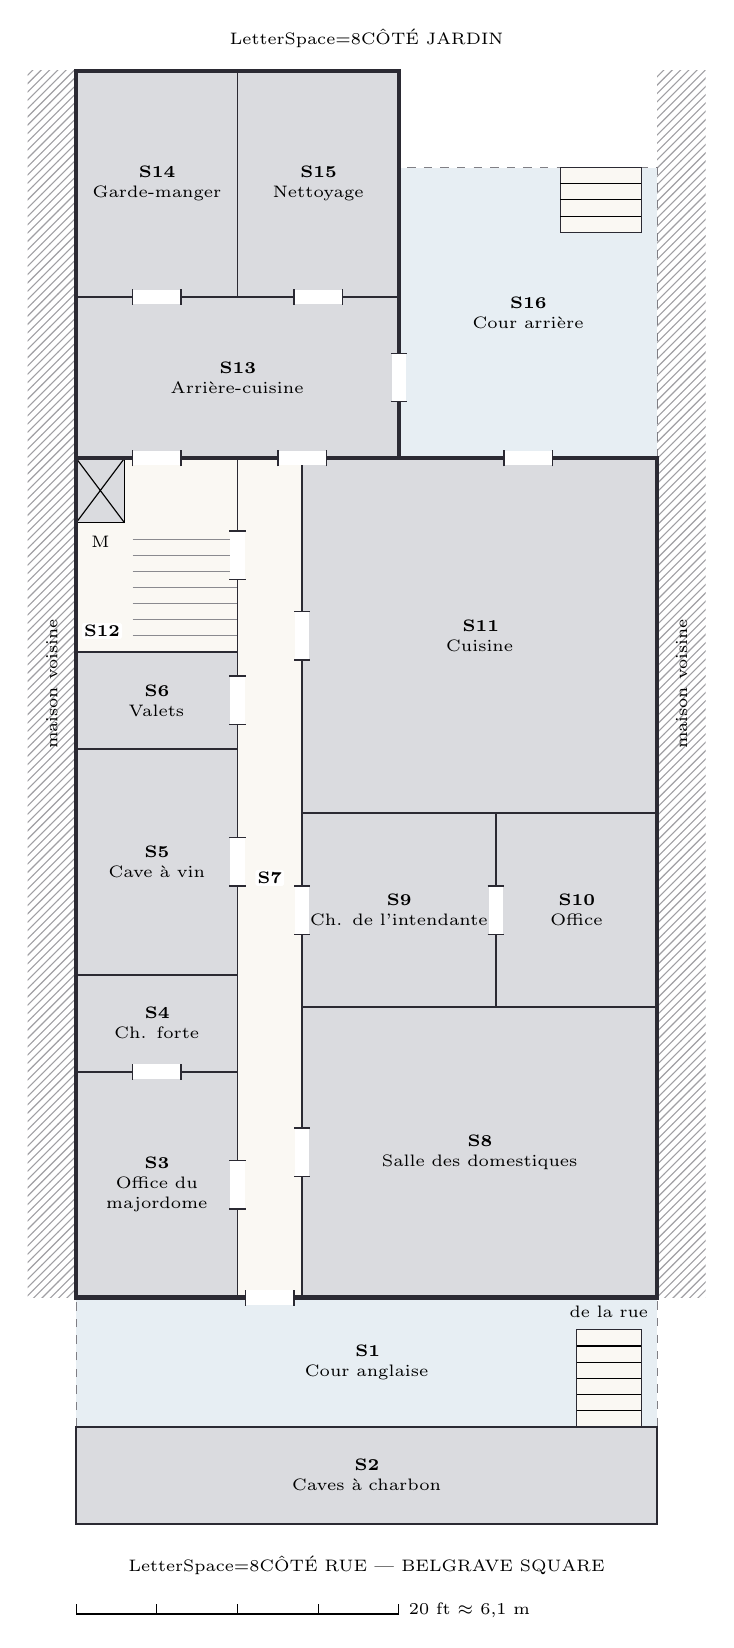
\begin{tikzpicture}[x=0.205cm,y=0.205cm]
\fill[pattern=north east lines, pattern color=wallc!45] (-3,0) rectangle (0,76);
\fill[pattern=north east lines, pattern color=wallc!45] (36,0) rectangle (39,76);
\node[tiny,rotate=90] at (-1.5,38) {maison voisine};
\node[tiny,rotate=90] at (37.5,38) {maison voisine};
\node[tiny] at (18,-16.6) {\caps{côté rue — Belgrave Square}};
\node[tiny] at (18,78) {\caps{côté jardin}};
\fill[ext] (0,-8) rectangle (36,0);
\fill[srv] (0,-14) rectangle (36,-8);
\fill[srv] (0,0) rectangle (10,14);
\fill[srv] (0,14) rectangle (10,20);
\fill[srv] (0,20) rectangle (10,34);
\fill[srv] (0,34) rectangle (10,40);
\fill[cir] (10,0) rectangle (14,52);
\fill[srv] (14,0) rectangle (36,18);
\fill[srv] (14,18) rectangle (26,30);
\fill[srv] (26,18) rectangle (36,30);
\fill[srv] (14,30) rectangle (36,52);
\fill[cir] (0,40) rectangle (10,52);
\fill[srv] (0,52) rectangle (20,62);
\fill[srv] (0,62) rectangle (10,76);
\fill[srv] (10,62) rectangle (20,76);
\fill[ext] (20,52) rectangle (36,70);
\fill[cir] (0,40) rectangle (10,52);
\draw[tread] (3.5,41) -- (10,41);
\draw[tread] (3.5,42) -- (10,42);
\draw[tread] (3.5,43) -- (10,43);
\draw[tread] (3.5,44) -- (10,44);
\draw[tread] (3.5,45) -- (10,45);
\draw[tread] (3.5,46) -- (10,46);
\draw[tread] (3.5,47) -- (10,47);
\fill[srv] (0,48) rectangle (3,52); \draw[thin] (0,48) rectangle (3,52);
\draw[thin] (0,48) -- (3,52) (0,52) -- (3,48);
\node[tiny] at (1.5,46.8) {M};
\draw[extwall] (0,-8) rectangle (36,0);
\draw[wall] (0,-14) rectangle (36,-8);
\draw[wall] (0,0) rectangle (10,14);
\draw[wall] (0,14) rectangle (10,20);
\draw[wall] (0,20) rectangle (10,34);
\draw[wall] (0,34) rectangle (10,40);
\draw[wall] (10,0) rectangle (14,52);
\draw[wall] (14,0) rectangle (36,18);
\draw[wall] (14,18) rectangle (26,30);
\draw[wall] (26,18) rectangle (36,30);
\draw[wall] (14,30) rectangle (36,52);
\draw[wall] (0,40) rectangle (10,52);
\draw[wall] (0,52) rectangle (20,62);
\draw[wall] (0,62) rectangle (10,76);
\draw[wall] (10,62) rectangle (20,76);
\draw[extwall] (20,52) rectangle (36,70);
\draw[outer] (0,0) rectangle (36,52);
\draw[outer] (0,52) -- (0,76) -- (20,76) -- (20,52);
\draw[stair] (31,-8) rectangle (35,-2); \foreach \i in {-7,...,-3} \draw[thin] (31,\i) -- (35,\i); \node[tiny] at (33,-0.9) {de la rue};
\draw[stair] (30,66) rectangle (35,70); \foreach \i in {67,68,69} \draw[thin] (30,\i) -- (35,\i);
\fill[white] (9.55,5.5) rectangle (10.45,8.5);
\draw[jamb] (9.5,5.5) -- (10.5,5.5) (9.5,8.5) -- (10.5,8.5);
\fill[white] (3.5,13.55) rectangle (6.5,14.45);
\draw[jamb] (3.5,13.5) -- (3.5,14.5) (6.5,13.5) -- (6.5,14.5);
\fill[white] (9.55,25.5) rectangle (10.45,28.5);
\draw[jamb] (9.5,25.5) -- (10.5,25.5) (9.5,28.5) -- (10.5,28.5);
\fill[white] (9.55,35.5) rectangle (10.45,38.5);
\draw[jamb] (9.5,35.5) -- (10.5,35.5) (9.5,38.5) -- (10.5,38.5);
\fill[white] (13.55,7.5) rectangle (14.45,10.5);
\draw[jamb] (13.5,7.5) -- (14.5,7.5) (13.5,10.5) -- (14.5,10.5);
\fill[white] (13.55,22.5) rectangle (14.45,25.5);
\draw[jamb] (13.5,22.5) -- (14.5,22.5) (13.5,25.5) -- (14.5,25.5);
\fill[white] (25.55,22.5) rectangle (26.45,25.5);
\draw[jamb] (25.5,22.5) -- (26.5,22.5) (25.5,25.5) -- (26.5,25.5);
\fill[white] (13.55,39.5) rectangle (14.45,42.5);
\draw[jamb] (13.5,39.5) -- (14.5,39.5) (13.5,42.5) -- (14.5,42.5);
\fill[white] (9.55,44.5) rectangle (10.45,47.5);
\draw[jamb] (9.5,44.5) -- (10.5,44.5) (9.5,47.5) -- (10.5,47.5);
\fill[white] (3.5,51.55) rectangle (6.5,52.45);
\draw[jamb] (3.5,51.5) -- (3.5,52.5) (6.5,51.5) -- (6.5,52.5);
\fill[white] (12.5,51.55) rectangle (15.5,52.45);
\draw[jamb] (12.5,51.5) -- (12.5,52.5) (15.5,51.5) -- (15.5,52.5);
\fill[white] (3.5,61.55) rectangle (6.5,62.45);
\draw[jamb] (3.5,61.5) -- (3.5,62.5) (6.5,61.5) -- (6.5,62.5);
\fill[white] (13.5,61.55) rectangle (16.5,62.45);
\draw[jamb] (13.5,61.5) -- (13.5,62.5) (16.5,61.5) -- (16.5,62.5);
\fill[white] (19.55,55.5) rectangle (20.45,58.5);
\draw[jamb] (19.5,55.5) -- (20.5,55.5) (19.5,58.5) -- (20.5,58.5);
\fill[white] (26.5,51.55) rectangle (29.5,52.45);
\draw[jamb] (26.5,51.5) -- (26.5,52.5) (29.5,51.5) -- (29.5,52.5);
\fill[white] (10.5,-0.45) rectangle (13.5,0.45);
\draw[jamb] (10.5,-0.5) -- (10.5,0.5) (13.5,-0.5) -- (13.5,0.5);
\node[lab, text width=7.23cm] at (18,-4) {\textbf{S1}\\ Cour anglaise};
\node[lab, text width=7.23cm] at (18,-11) {\textbf{S2}\\ Caves à charbon};
\node[lab, text width=1.90cm] at (5,7) {\textbf{S3}\\ Office du majordome};
\node[lab, text width=1.90cm] at (5,17) {\textbf{S4}\\ Ch. forte};
\node[lab, text width=1.90cm] at (5,27) {\textbf{S5}\\ Cave à vin};
\node[lab, text width=1.90cm] at (5,37) {\textbf{S6}\\ Valets};
\node[lab, text width=4.36cm] at (25,9) {\textbf{S8}\\ Salle des domestiques};
\node[lab, text width=2.31cm] at (20,24) {\textbf{S9}\\ Ch. de l'intendante};
\node[lab, text width=1.90cm] at (31,24) {\textbf{S10}\\ Office};
\node[lab, text width=4.36cm] at (25,41) {\textbf{S11}\\ Cuisine};
\node[lab, text width=3.95cm] at (10,57) {\textbf{S13}\\ Arrière-cuisine};
\node[lab, text width=1.90cm] at (5,69) {\textbf{S14}\\ Garde-manger};
\node[lab, text width=1.90cm] at (15,69) {\textbf{S15}\\ Nettoyage};
\node[lab, text width=3.13cm] at (28,61) {\textbf{S16}\\ Cour arrière};
\node[numtag] at (12,26) {S7};
\node[numtag] at (1.6,41.3) {S12};
\begin{scope}[shift={(0,-19.6)}]
\draw[thin] (0,0) -- (20,0); \foreach \i in {0,5,...,20} \draw[thin] (\i,0) -- (\i,0.6);
\node[tiny,anchor=west] at (20.5,0.2) {20 ft $\approx$ 6,1 m};
\end{scope}
\end{tikzpicture}
\end{minipage}\hfill\begin{minipage}[t]{8.95cm}\vspace{0pt}\fontsize{8.4}{10.2}\selectfont
\begin{descr}
\item[\textbf{S1}] \textbf{Cour anglaise (area)}. Fossé de 8 ft entre le trottoir et la façade, fermé par une grille en fer forgé. Un escalier raide y descend depuis la rue : c'est l'entrée des fournisseurs et des domestiques. Les fenêtres du sous-sol donnent dessus.
\item[\textbf{S2}] \textbf{Caves à charbon (sous le trottoir)}. Trois voûtes creusées sous le trottoir. On y déverse le charbon depuis la rue par des trappes rondes en fonte. Il alimente le fourneau de la cuisine et toutes les cheminées de la maison.
\item[\textbf{S3}] \textbf{Office du majordome}. Le poste de commandement du majordome, près de l'entrée de service pour surveiller les allées et venues. On y lave et on y range la verrerie fine et l'argenterie, et c'est là qu'on prépare les plateaux. Il y dort dans un lit pliant, à côté de la chambre forte, comme le veut l'usage. \textit{Ce soir :} c'est ici que le verre destiné à Marcus est préparé.
\item[\textbf{S4}] \textbf{Chambre forte de l'argenterie}. Petite pièce à porte de fer, sans fenêtre, accessible seulement depuis l'office du majordome. On y garde l'argenterie de famille et les plats d'apparat.
\item[\textbf{S5}] \textbf{Cave à vin}. Voûtée, fraîche, fermée à clé ; seul le majordome en détient la clé. Casiers à bouteilles, fûts de bière dans un recoin.
\item[\textbf{S6}] \textbf{Chambre des valets de pied}. Deux lits étroits pour les deux valets de pied. Kerr prévoit au sous-sol « a sleeping room for two menservants », pour que les hommes ne dorment pas sous les toits avec les servantes.
\item[\textbf{S7}] \textbf{Couloir de service}. Long couloir dallé de pierre qui dessert tout le sous-sol, de l'entrée de service jusqu'à l'escalier de service. Mal éclairé, il sent le charbon et la cuisine.
\item[\textbf{S8}] \textbf{Salle des domestiques (servants' hall)}. Grande table de bois brut où les domestiques prennent leurs repas, selon une stricte hiérarchie : le majordome préside, l'intendante en face. Un tableau de sonnettes au mur indique de quelle pièce on appelle.
\item[\textbf{S9}] \textbf{Chambre de l'intendante}. Le salon privé de Mrs. Hartwell, intendante et gouvernante en chef depuis 25 ans : fauteuil, bureau aux livres de comptes, clés de la maison. Ce soir la pièce est vide, puisqu'elle est retenue au manoir.
\item[\textbf{S10}] \textbf{Office (still-room)}. Domaine de l'intendante : confitures, conserves, thé, café, gâteaux secs. On y prépare ce qui n'est pas de la cuisine proprement dite.
\item[\textbf{S11}] \textbf{Cuisine}. Grande pièce haute, carrelée, avec un fourneau fermé en fonte (le « range ») et sa chaudière arrière qui chauffe l'eau de la maison. Batterie de cuivre au mur, horloge des domestiques au-dessus de la porte. Les fenêtres donnent sur la cour arrière. \textit{Ce soir :} la cuisinière et ses aides y préparent le buffet.
\item[\textbf{S12}] \textbf{Escalier de service et monte-charge}. Escalier étroit qui monte du sous-sol aux combles, réservé aux domestiques. Kerr y place un monte-charge : « The Back-stair has a Lift from bottom to top. » C'est par là que les plats et la verrerie montent vers la salle à manger.
\item[\textbf{S13}] \textbf{Arrière-cuisine (scullery)}. Éviers de pierre, eau froide, vaisselle sale. Le domaine de la fille de cuisine la plus jeune.
\item[\textbf{S14}] \textbf{Garde-manger (larder)}. Pièce fraîche, orientée au nord, avec étagères de pierre et garde-manger grillagé pour la viande et le gibier.
\item[\textbf{S15}] \textbf{Salle de nettoyage}. On y cire les bottes, on y aiguise les couteaux et on y entretient les lampes et les becs de gaz.
\item[\textbf{S16}] \textbf{Cour arrière}. Cour dallée en contrebas, au niveau du sous-sol. Elle éclaire la cuisine et l'arrière-cuisine. Quelques marches remontent vers le jardin. Le jardin d'hiver du premier étage la surplombe.
\end{descr}
\end{minipage}
\newpage
\niveau{Rez-de-chaussée — l'accueil et le buffet}
{\small\textit{Hauteur : env. 14 ft sous plafond (4,25 m) ; surélevé de quelques marches au-dessus de la rue.}}\par
{\small L'étage qu'on traverse en arrivant. Suivant Kerr, la salle à manger est à l'arrière, « as it ought to be, if possible », et la bibliothèque, « necessarily small », donne sur la rue. Ce soir, la salle à manger accueille le buffet.}\par\vspace{4pt}
\noindent\begin{minipage}[t]{8.75cm}\vspace{0pt}
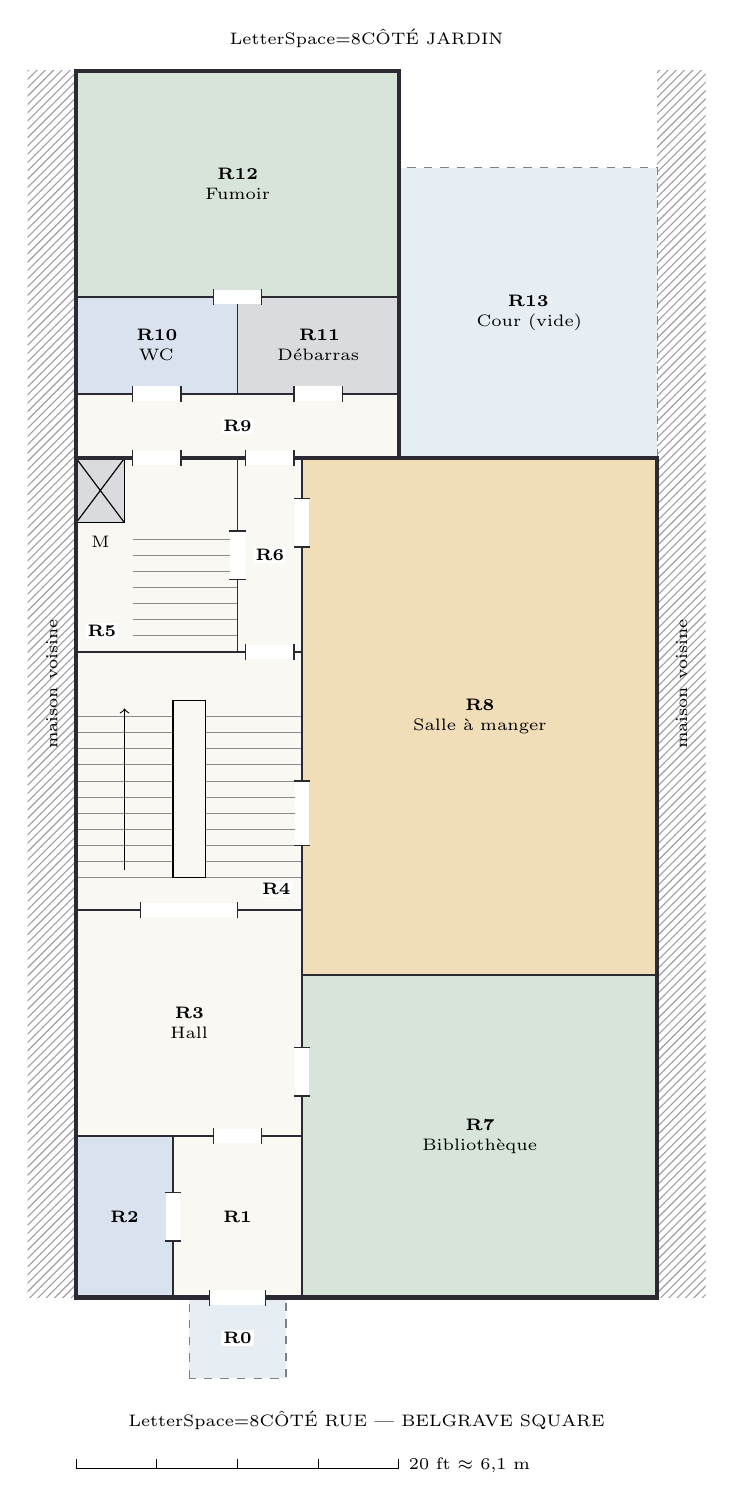
\begin{tikzpicture}[x=0.205cm,y=0.205cm]
\fill[pattern=north east lines, pattern color=wallc!45] (-3,0) rectangle (0,76);
\fill[pattern=north east lines, pattern color=wallc!45] (36,0) rectangle (39,76);
\node[tiny,rotate=90] at (-1.5,38) {maison voisine};
\node[tiny,rotate=90] at (37.5,38) {maison voisine};
\node[tiny] at (18,-7.6) {\caps{côté rue — Belgrave Square}};
\node[tiny] at (18,78) {\caps{côté jardin}};
\fill[ext] (7,-5) rectangle (13,0);
\fill[cir] (6,0) rectangle (14,10);
\fill[san] (0,0) rectangle (6,10);
\fill[cir] (0,10) rectangle (14,24);
\fill[cir] (0,24) rectangle (14,40);
\fill[cir] (0,40) rectangle (10,52);
\fill[cir] (10,40) rectangle (14,52);
\fill[fam] (14,0) rectangle (36,20);
\fill[rec] (14,20) rectangle (36,52);
\fill[cir] (0,52) rectangle (20,56);
\fill[san] (0,56) rectangle (10,62);
\fill[srv] (10,56) rectangle (20,62);
\fill[fam] (0,62) rectangle (20,76);
\fill[ext] (20,52) rectangle (36,70);
\fill[cir] (0,24) rectangle (14,40);
\draw[tread] (0,26) -- (6.0,26);
\draw[tread] (8.0,26) -- (14,26);
\draw[tread] (0,27) -- (6.0,27);
\draw[tread] (8.0,27) -- (14,27);
\draw[tread] (0,28) -- (6.0,28);
\draw[tread] (8.0,28) -- (14,28);
\draw[tread] (0,29) -- (6.0,29);
\draw[tread] (8.0,29) -- (14,29);
\draw[tread] (0,30) -- (6.0,30);
\draw[tread] (8.0,30) -- (14,30);
\draw[tread] (0,31) -- (6.0,31);
\draw[tread] (8.0,31) -- (14,31);
\draw[tread] (0,32) -- (6.0,32);
\draw[tread] (8.0,32) -- (14,32);
\draw[tread] (0,33) -- (6.0,33);
\draw[tread] (8.0,33) -- (14,33);
\draw[tread] (0,34) -- (6.0,34);
\draw[tread] (8.0,34) -- (14,34);
\draw[tread] (0,35) -- (6.0,35);
\draw[tread] (8.0,35) -- (14,35);
\draw[tread] (0,36) -- (6.0,36);
\draw[tread] (8.0,36) -- (14,36);
\draw[thin] (6.0,26) rectangle (8.0,37);
\draw[->,thin] (3.0,26.5) -- (3.0,36.5);
\fill[cir] (0,40) rectangle (10,52);
\draw[tread] (3.5,41) -- (10,41);
\draw[tread] (3.5,42) -- (10,42);
\draw[tread] (3.5,43) -- (10,43);
\draw[tread] (3.5,44) -- (10,44);
\draw[tread] (3.5,45) -- (10,45);
\draw[tread] (3.5,46) -- (10,46);
\draw[tread] (3.5,47) -- (10,47);
\fill[srv] (0,48) rectangle (3,52); \draw[thin] (0,48) rectangle (3,52);
\draw[thin] (0,48) -- (3,52) (0,52) -- (3,48);
\node[tiny] at (1.5,46.8) {M};
\draw[extwall] (7,-5) rectangle (13,0);
\draw[wall] (6,0) rectangle (14,10);
\draw[wall] (0,0) rectangle (6,10);
\draw[wall] (0,10) rectangle (14,24);
\draw[wall] (0,24) rectangle (14,40);
\draw[wall] (0,40) rectangle (10,52);
\draw[wall] (10,40) rectangle (14,52);
\draw[wall] (14,0) rectangle (36,20);
\draw[wall] (14,20) rectangle (36,52);
\draw[wall] (0,52) rectangle (20,56);
\draw[wall] (0,56) rectangle (10,62);
\draw[wall] (10,56) rectangle (20,62);
\draw[wall] (0,62) rectangle (20,76);
\draw[extwall] (20,52) rectangle (36,70);
\draw[outer] (0,0) rectangle (36,52);
\draw[outer] (0,52) -- (0,76) -- (20,76) -- (20,52);
\fill[white] (8.25,-0.45) rectangle (11.75,0.45);
\draw[jamb] (8.25,-0.5) -- (8.25,0.5) (11.75,-0.5) -- (11.75,0.5);
\fill[white] (5.55,3.5) rectangle (6.45,6.5);
\draw[jamb] (5.5,3.5) -- (6.5,3.5) (5.5,6.5) -- (6.5,6.5);
\fill[white] (8.5,9.55) rectangle (11.5,10.45);
\draw[jamb] (8.5,9.5) -- (8.5,10.5) (11.5,9.5) -- (11.5,10.5);
\fill[white] (13.55,12.5) rectangle (14.45,15.5);
\draw[jamb] (13.5,12.5) -- (14.5,12.5) (13.5,15.5) -- (14.5,15.5);
\fill[white] (4,23.55) rectangle (10,24.45);
\draw[jamb] (4,23.5) -- (4,24.5) (10,23.5) -- (10,24.5);
\fill[white] (13.55,28) rectangle (14.45,32);
\draw[jamb] (13.5,28) -- (14.5,28) (13.5,32) -- (14.5,32);
\fill[white] (10.5,39.55) rectangle (13.5,40.45);
\draw[jamb] (10.5,39.5) -- (10.5,40.5) (13.5,39.5) -- (13.5,40.5);
\fill[white] (13.55,46.5) rectangle (14.45,49.5);
\draw[jamb] (13.5,46.5) -- (14.5,46.5) (13.5,49.5) -- (14.5,49.5);
\fill[white] (9.55,44.5) rectangle (10.45,47.5);
\draw[jamb] (9.5,44.5) -- (10.5,44.5) (9.5,47.5) -- (10.5,47.5);
\fill[white] (3.5,51.55) rectangle (6.5,52.45);
\draw[jamb] (3.5,51.5) -- (3.5,52.5) (6.5,51.5) -- (6.5,52.5);
\fill[white] (10.5,51.55) rectangle (13.5,52.45);
\draw[jamb] (10.5,51.5) -- (10.5,52.5) (13.5,51.5) -- (13.5,52.5);
\fill[white] (3.5,55.55) rectangle (6.5,56.45);
\draw[jamb] (3.5,55.5) -- (3.5,56.5) (6.5,55.5) -- (6.5,56.5);
\fill[white] (13.5,55.55) rectangle (16.5,56.45);
\draw[jamb] (13.5,55.5) -- (13.5,56.5) (16.5,55.5) -- (16.5,56.5);
\fill[white] (8.5,61.55) rectangle (11.5,62.45);
\draw[jamb] (8.5,61.5) -- (8.5,62.5) (11.5,61.5) -- (11.5,62.5);
\node[lab] at (10,5) {\textbf{R1}};
\node[lab] at (3,5) {\textbf{R2}};
\node[lab, text width=2.72cm] at (7,17) {\textbf{R3}\\ Hall};
\node[lab, text width=4.36cm] at (25,10) {\textbf{R7}\\ Bibliothèque};
\node[lab, text width=4.36cm] at (25,36) {\textbf{R8}\\ Salle à manger};
\node[lab, text width=1.90cm] at (5,59) {\textbf{R10}\\ WC};
\node[lab, text width=1.90cm] at (15,59) {\textbf{R11}\\ Débarras};
\node[lab, text width=3.95cm] at (10,69) {\textbf{R12}\\ Fumoir};
\node[lab, text width=3.13cm] at (28,61) {\textbf{R13}\\ Cour (vide)};
\node[numtag] at (10,-2.5) {R0};
\node[numtag] at (12.4,25.3) {R4};
\node[numtag] at (1.6,41.3) {R5};
\node[numtag] at (12,46) {R6};
\node[numtag] at (10,54) {R9};
\begin{scope}[shift={(0,-10.6)}]
\draw[thin] (0,0) -- (20,0); \foreach \i in {0,5,...,20} \draw[thin] (\i,0) -- (\i,0.6);
\node[tiny,anchor=west] at (20.5,0.2) {20 ft $\approx$ 6,1 m};
\end{scope}
\end{tikzpicture}
\end{minipage}\hfill\begin{minipage}[t]{8.95cm}\vspace{0pt}\fontsize{8.4}{10.2}\selectfont
\begin{descr}
\item[\textbf{R0}] \textbf{Perron}. Quelques marches de pierre franchissent la cour anglaise jusqu'à la porte d'entrée, sous un porche à deux colonnes. Façade en stuc blanc, typique des terraces de Belgravia.
\item[\textbf{R1}] \textbf{Vestibule}. Sas entre la porte d'entrée et le hall. Le valet de pied y reçoit les invités et y annonce leur arrivée. Sol de marbre en damier noir et blanc.
\item[\textbf{R2}] \textbf{Vestiaire et lavabo des messieurs}. On y dépose manteaux, cannes et chapeaux haut de forme. Lavabo et cabinet d'aisances à chasse d'eau.
\item[\textbf{R3}] \textbf{Hall d'entrée}. Hall dallé, cheminée, banquette, porte-parapluies. Contre le mur se dresse la grande horloge de parquet : c'est elle qui donne l'heure de la maison et qui sonne les heures. \textit{Ce soir :} c'est l'horloge que Vivienne entend.
\item[\textbf{R4}] \textbf{Grand escalier}. Escalier d'apparat en pierre, tapis retenu par des tringles de laiton, rampe d'acajou. Il monte jusqu'au troisième étage. Une verrière, au sommet de la cage, l'éclaire de jour. (Clin d'œil à la vraie soirée : la quatrième marche.)
\item[\textbf{R5}] \textbf{Escalier de service}. Arrivée du monte-charge. Un domestique y réceptionne plats et verrerie avant de les porter à la salle à manger.
\item[\textbf{R6}] \textbf{Couloir arrière et desserte}. Passage étroit entre l'escalier de service et la salle à manger. Une console sert d'office de desserte : on y pose les plateaux avant le service. C'est le « Service-closet for the Dining-room » de Kerr.
\item[\textbf{R7}] \textbf{Bibliothèque}. Rayonnages d'acajou du sol au plafond, fauteuils de cuir, globe terrestre, grand bureau. C'est la pièce de Lord Whitmore quand il est à Londres. Fenêtres sur le square. (Clin d'œil à la vraie soirée : \emph{La Panthère des neiges} cachée dans les rayons.)
\item[\textbf{R8}] \textbf{Salle à manger}. La plus grande pièce du rez-de-chaussée : boiseries sombres, portraits de famille, lustre au gaz. La longue table d'acajou a été poussée contre le mur et sert de buffet. \textit{Ce soir :} buffet debout, champagne, va-et-vient permanent. C'est là que les invités se servent et que Béatrice trébuche.
\item[\textbf{R9}] \textbf{Passage}. Relie la maison principale à l'aile arrière.
\item[\textbf{R10}] \textbf{Toilettes}. Cabinet d'aisances à chasse d'eau, cuvette en faïence décorée. Les modèles tout en céramique se répandent depuis l'Exposition d'hygiène de 1884.
\item[\textbf{R11}] \textbf{Débarras}. Armoire à fusils de chasse, cannes, imperméables.
\item[\textbf{R12}] \textbf{Cabinet de Lord Whitmore (fumoir)}. Pièce d'homme sur le jardin : cuir, tabac, trophées, journaux. En l'absence de Lord Whitmore, elle sert de fumoir aux messieurs. \textit{Ce soir :} on s'y retire pour fumer, loin des dames.
\item[\textbf{R13}] \textbf{Cour arrière (en contrebas)}. Vue plongeante sur la cour du sous-sol.
\end{descr}
\end{minipage}
\newpage
\niveau{Premier étage — l'étage noble}
{\small\textit{Hauteur : env. 16 ft sous plafond (4,90 m) : le plus haut de la maison.}}\par
{\small L'étage de réception. Kerr y place « two spacious Drawing-rooms and a connecting Ante-room » ; ici, les portes pliantes entre les trois pièces s'ouvrent ce soir en une seule enfilade. Grandes fenêtres et balcon sur le square.}\par\vspace{4pt}
\noindent\begin{minipage}[t]{8.75cm}\vspace{0pt}
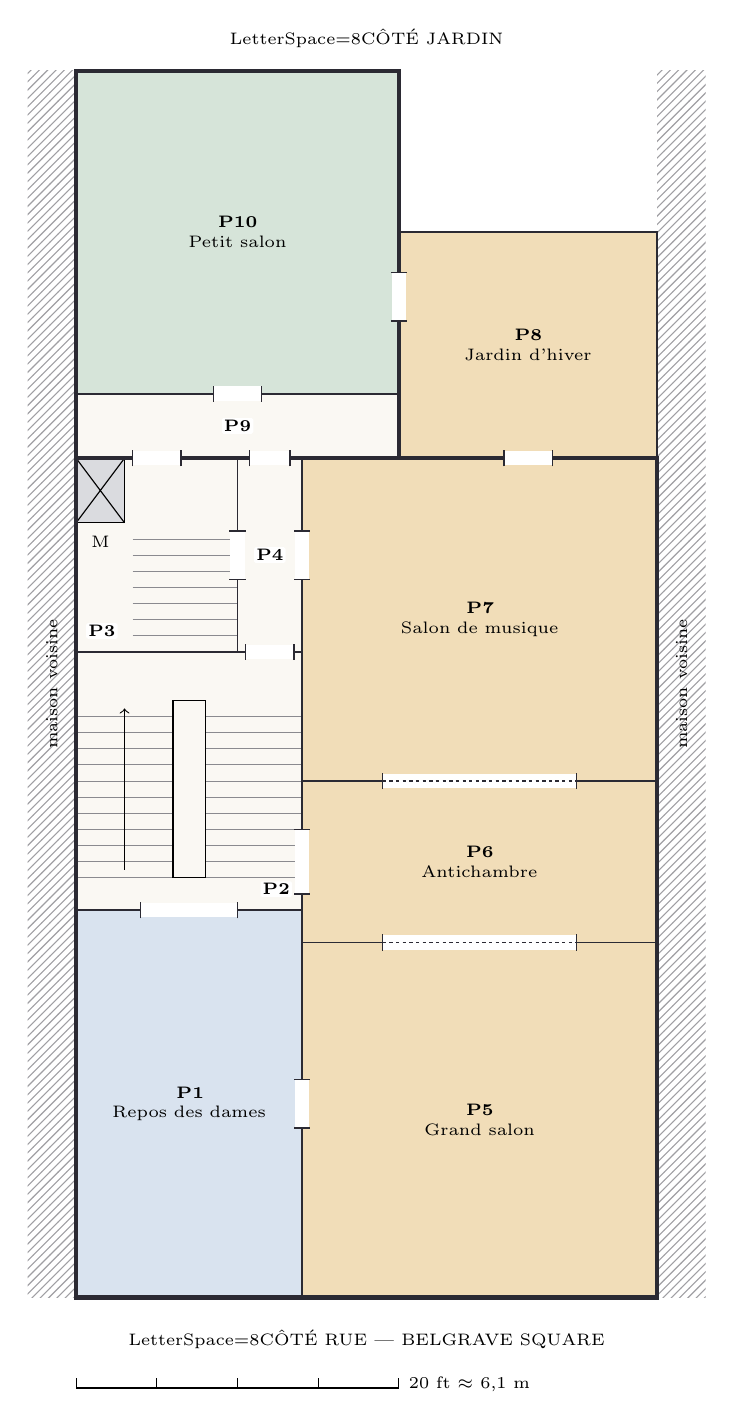
\begin{tikzpicture}[x=0.205cm,y=0.205cm]
\fill[pattern=north east lines, pattern color=wallc!45] (-3,0) rectangle (0,76);
\fill[pattern=north east lines, pattern color=wallc!45] (36,0) rectangle (39,76);
\node[tiny,rotate=90] at (-1.5,38) {maison voisine};
\node[tiny,rotate=90] at (37.5,38) {maison voisine};
\node[tiny] at (18,-2.6) {\caps{côté rue — Belgrave Square}};
\node[tiny] at (18,78) {\caps{côté jardin}};
\fill[san] (0,0) rectangle (14,24);
\fill[cir] (0,24) rectangle (14,40);
\fill[cir] (0,40) rectangle (10,52);
\fill[cir] (10,40) rectangle (14,52);
\fill[rec] (14,0) rectangle (36,22);
\fill[rec] (14,22) rectangle (36,32);
\fill[rec] (14,32) rectangle (36,52);
\fill[rec] (20,52) rectangle (36,66);
\fill[cir] (0,52) rectangle (20,56);
\fill[fam] (0,56) rectangle (20,76);
\fill[cir] (0,24) rectangle (14,40);
\draw[tread] (0,26) -- (6.0,26);
\draw[tread] (8.0,26) -- (14,26);
\draw[tread] (0,27) -- (6.0,27);
\draw[tread] (8.0,27) -- (14,27);
\draw[tread] (0,28) -- (6.0,28);
\draw[tread] (8.0,28) -- (14,28);
\draw[tread] (0,29) -- (6.0,29);
\draw[tread] (8.0,29) -- (14,29);
\draw[tread] (0,30) -- (6.0,30);
\draw[tread] (8.0,30) -- (14,30);
\draw[tread] (0,31) -- (6.0,31);
\draw[tread] (8.0,31) -- (14,31);
\draw[tread] (0,32) -- (6.0,32);
\draw[tread] (8.0,32) -- (14,32);
\draw[tread] (0,33) -- (6.0,33);
\draw[tread] (8.0,33) -- (14,33);
\draw[tread] (0,34) -- (6.0,34);
\draw[tread] (8.0,34) -- (14,34);
\draw[tread] (0,35) -- (6.0,35);
\draw[tread] (8.0,35) -- (14,35);
\draw[tread] (0,36) -- (6.0,36);
\draw[tread] (8.0,36) -- (14,36);
\draw[thin] (6.0,26) rectangle (8.0,37);
\draw[->,thin] (3.0,26.5) -- (3.0,36.5);
\fill[cir] (0,40) rectangle (10,52);
\draw[tread] (3.5,41) -- (10,41);
\draw[tread] (3.5,42) -- (10,42);
\draw[tread] (3.5,43) -- (10,43);
\draw[tread] (3.5,44) -- (10,44);
\draw[tread] (3.5,45) -- (10,45);
\draw[tread] (3.5,46) -- (10,46);
\draw[tread] (3.5,47) -- (10,47);
\fill[srv] (0,48) rectangle (3,52); \draw[thin] (0,48) rectangle (3,52);
\draw[thin] (0,48) -- (3,52) (0,52) -- (3,48);
\node[tiny] at (1.5,46.8) {M};
\draw[wall] (0,0) rectangle (14,24);
\draw[wall] (0,24) rectangle (14,40);
\draw[wall] (0,40) rectangle (10,52);
\draw[wall] (10,40) rectangle (14,52);
\draw[wall] (14,0) rectangle (36,22);
\draw[wall] (14,22) rectangle (36,32);
\draw[wall] (14,32) rectangle (36,52);
\draw[wall] (20,52) rectangle (36,66);
\draw[wall] (0,52) rectangle (20,56);
\draw[wall] (0,56) rectangle (20,76);
\draw[outer] (0,0) rectangle (36,52);
\draw[outer] (0,52) -- (0,76) -- (20,76) -- (20,52);
\fill[white] (4,23.55) rectangle (10,24.45);
\draw[jamb] (4,23.5) -- (4,24.5) (10,23.5) -- (10,24.5);
\fill[white] (13.55,25) rectangle (14.45,29);
\draw[jamb] (13.5,25) -- (14.5,25) (13.5,29) -- (14.5,29);
\fill[white] (13.55,10.5) rectangle (14.45,13.5);
\draw[jamb] (13.5,10.5) -- (14.5,10.5) (13.5,13.5) -- (14.5,13.5);
\fill[white] (19,21.55) rectangle (31,22.45);
\draw[jamb] (19,21.5) -- (19,22.5) (31,21.5) -- (31,22.5);
\draw[fold] (19,22) -- (31,22);
\fill[white] (19,31.55) rectangle (31,32.45);
\draw[jamb] (19,31.5) -- (19,32.5) (31,31.5) -- (31,32.5);
\draw[fold] (19,32) -- (31,32);
\fill[white] (10.5,39.55) rectangle (13.5,40.45);
\draw[jamb] (10.5,39.5) -- (10.5,40.5) (13.5,39.5) -- (13.5,40.5);
\fill[white] (13.55,44.5) rectangle (14.45,47.5);
\draw[jamb] (13.5,44.5) -- (14.5,44.5) (13.5,47.5) -- (14.5,47.5);
\fill[white] (9.55,44.5) rectangle (10.45,47.5);
\draw[jamb] (9.5,44.5) -- (10.5,44.5) (9.5,47.5) -- (10.5,47.5);
\fill[white] (26.5,51.55) rectangle (29.5,52.45);
\draw[jamb] (26.5,51.5) -- (26.5,52.5) (29.5,51.5) -- (29.5,52.5);
\fill[white] (3.5,51.55) rectangle (6.5,52.45);
\draw[jamb] (3.5,51.5) -- (3.5,52.5) (6.5,51.5) -- (6.5,52.5);
\fill[white] (10.75,51.55) rectangle (13.25,52.45);
\draw[jamb] (10.75,51.5) -- (10.75,52.5) (13.25,51.5) -- (13.25,52.5);
\fill[white] (8.5,55.55) rectangle (11.5,56.45);
\draw[jamb] (8.5,55.5) -- (8.5,56.5) (11.5,55.5) -- (11.5,56.5);
\fill[white] (19.55,60.5) rectangle (20.45,63.5);
\draw[jamb] (19.5,60.5) -- (20.5,60.5) (19.5,63.5) -- (20.5,63.5);
\node[lab, text width=2.72cm] at (7,12) {\textbf{P1}\\ Repos des dames};
\node[lab, text width=4.36cm] at (25,11) {\textbf{P5}\\ Grand salon};
\node[lab, text width=4.36cm] at (25,27) {\textbf{P6}\\ Antichambre};
\node[lab, text width=4.36cm] at (25,42) {\textbf{P7}\\ Salon de musique};
\node[lab, text width=3.13cm] at (28,59) {\textbf{P8}\\ Jardin d'hiver};
\node[lab, text width=3.95cm] at (10,66) {\textbf{P10}\\ Petit salon};
\node[numtag] at (12.4,25.3) {P2};
\node[numtag] at (1.6,41.3) {P3};
\node[numtag] at (12,46) {P4};
\node[numtag] at (10,54) {P9};
\begin{scope}[shift={(0,-5.6)}]
\draw[thin] (0,0) -- (20,0); \foreach \i in {0,5,...,20} \draw[thin] (\i,0) -- (\i,0.6);
\node[tiny,anchor=west] at (20.5,0.2) {20 ft $\approx$ 6,1 m};
\end{scope}
\end{tikzpicture}
\end{minipage}\hfill\begin{minipage}[t]{8.95cm}\vspace{0pt}\fontsize{8.4}{10.2}\selectfont
\begin{descr}
\item[\textbf{P1}] \textbf{Salon de repos des dames}. Pièce attenante aux salons où les dames se recoiffent et rajustent leur toilette : coiffeuse, grands miroirs, sofa, lavabo. Un cabinet d'aisances y est ménagé. (Clin d'œil : le miroir de la vraie soirée.) \textit{Ce soir :} c'est là que Béatrice demande qu'on l'emmène.
\item[\textbf{P2}] \textbf{Palier du grand escalier}. Large palier d'où l'on entre dans l'antichambre. Les invités y patientent et s'y croisent.
\item[\textbf{P3}] \textbf{Escalier de service}. Porte dérobée, tapissée comme le mur.
\item[\textbf{P4}] \textbf{Galerie}. Couloir qui mène à l'aile arrière et au petit salon, et que les domestiques empruntent pour rejoindre le salon de musique.
\item[\textbf{P5}] \textbf{Grand salon}. Le salon d'apparat sur le square : soieries, dorures, miroirs au-dessus de la cheminée, meubles et bibelots en abondance comme le veut le goût du temps. Trois hautes fenêtres ouvrent sur un balcon.
\item[\textbf{P6}] \textbf{Antichambre}. Pièce de liaison de 10 ft de large, la largeur que Kerr juge suffisante. Tables de jeu, fauteuils. \textit{Ce soir :} on y joue aux cartes et on y bavarde, à l'écart de la musique.
\item[\textbf{P7}] \textbf{Salon de musique}. Le cœur de la soirée : piano à queue Broadwood, chaises dorées en rangées, partitions sur un guéridon. L'acoustique est soignée. \textit{Ce soir :} le duo des Perles de Londres y chante.
\item[\textbf{P8}] \textbf{Jardin d'hiver}. Serre de fer et de verre accolée au salon de musique, suspendue au-dessus de la cour : palmiers en pots, fougères, orchidées, bancs d'osier. Chaleur humide, lumière tamisée. Le lieu classique des conversations à l'écart.
\item[\textbf{P9}] \textbf{Passage}. Mène de la galerie au petit salon.
\item[\textbf{P10}] \textbf{Petit salon}. Salon intime sur le jardin, loin du bruit de la réception : cheminée, deux fauteuils face à face, bougies. Une porte vitrée donne sur le jardin d'hiver. \textit{Ce soir :} la confession de Cordelia à Ophelia et Theodore (journal de Cordelia).
\end{descr}
\end{minipage}
\newpage
\niveau{Deuxième étage — les maîtres de maison}
{\small\textit{Hauteur : env. 12 ft sous plafond (3,65 m).}}\par
{\small Les appartements privés de Lord et Lady Whitmore, et l'appartement des invités. Kerr y prévoit « two complete Private Bedroom-Suites, one for the heads of the family and one for guests » et une salle de bain.}\par\vspace{4pt}
\noindent\begin{minipage}[t]{8.75cm}\vspace{0pt}
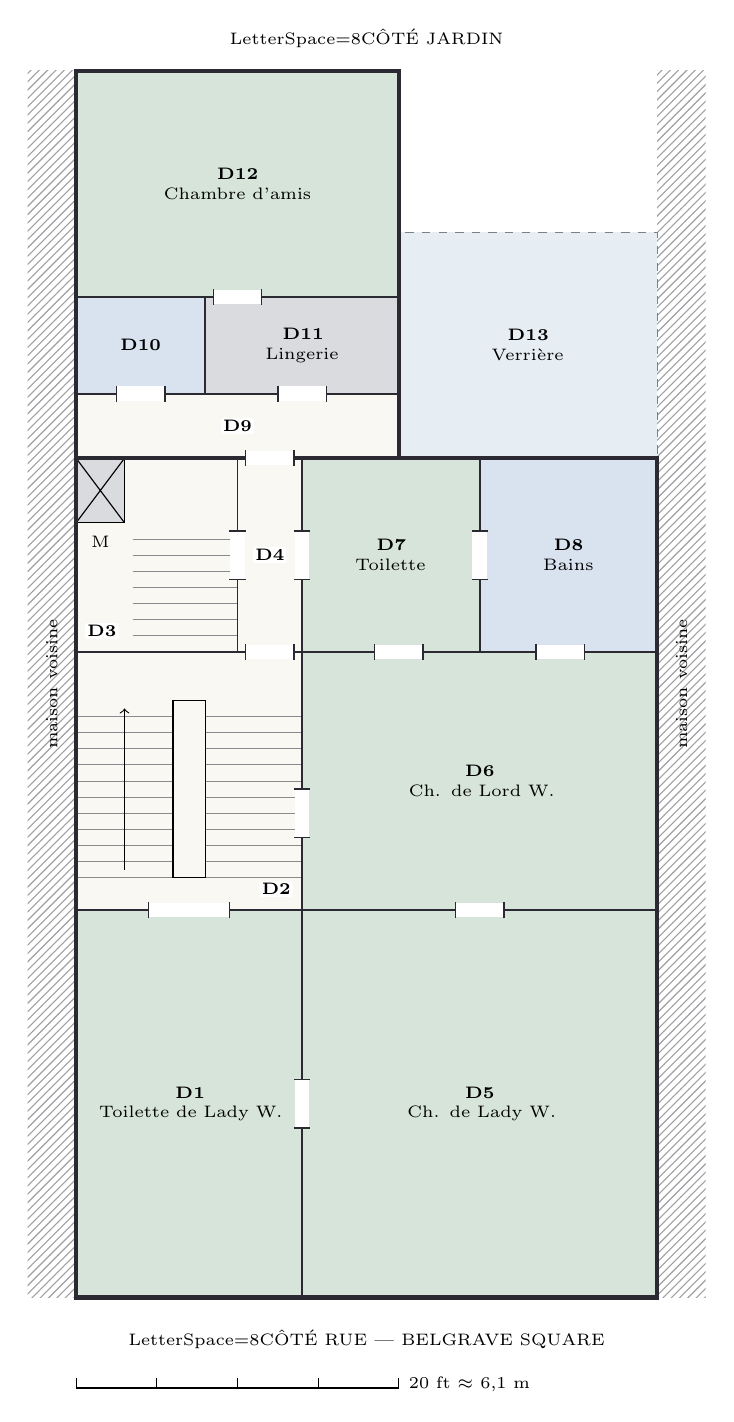
\begin{tikzpicture}[x=0.205cm,y=0.205cm]
\fill[pattern=north east lines, pattern color=wallc!45] (-3,0) rectangle (0,76);
\fill[pattern=north east lines, pattern color=wallc!45] (36,0) rectangle (39,76);
\node[tiny,rotate=90] at (-1.5,38) {maison voisine};
\node[tiny,rotate=90] at (37.5,38) {maison voisine};
\node[tiny] at (18,-2.6) {\caps{côté rue — Belgrave Square}};
\node[tiny] at (18,78) {\caps{côté jardin}};
\fill[fam] (0,0) rectangle (14,24);
\fill[cir] (0,24) rectangle (14,40);
\fill[cir] (0,40) rectangle (10,52);
\fill[cir] (10,40) rectangle (14,52);
\fill[fam] (14,0) rectangle (36,24);
\fill[fam] (14,24) rectangle (36,40);
\fill[fam] (14,40) rectangle (25,52);
\fill[san] (25,40) rectangle (36,52);
\fill[cir] (0,52) rectangle (20,56);
\fill[san] (0,56) rectangle (8,62);
\fill[srv] (8,56) rectangle (20,62);
\fill[fam] (0,62) rectangle (20,76);
\fill[ext] (20,52) rectangle (36,66);
\fill[cir] (0,24) rectangle (14,40);
\draw[tread] (0,26) -- (6.0,26);
\draw[tread] (8.0,26) -- (14,26);
\draw[tread] (0,27) -- (6.0,27);
\draw[tread] (8.0,27) -- (14,27);
\draw[tread] (0,28) -- (6.0,28);
\draw[tread] (8.0,28) -- (14,28);
\draw[tread] (0,29) -- (6.0,29);
\draw[tread] (8.0,29) -- (14,29);
\draw[tread] (0,30) -- (6.0,30);
\draw[tread] (8.0,30) -- (14,30);
\draw[tread] (0,31) -- (6.0,31);
\draw[tread] (8.0,31) -- (14,31);
\draw[tread] (0,32) -- (6.0,32);
\draw[tread] (8.0,32) -- (14,32);
\draw[tread] (0,33) -- (6.0,33);
\draw[tread] (8.0,33) -- (14,33);
\draw[tread] (0,34) -- (6.0,34);
\draw[tread] (8.0,34) -- (14,34);
\draw[tread] (0,35) -- (6.0,35);
\draw[tread] (8.0,35) -- (14,35);
\draw[tread] (0,36) -- (6.0,36);
\draw[tread] (8.0,36) -- (14,36);
\draw[thin] (6.0,26) rectangle (8.0,37);
\draw[->,thin] (3.0,26.5) -- (3.0,36.5);
\fill[cir] (0,40) rectangle (10,52);
\draw[tread] (3.5,41) -- (10,41);
\draw[tread] (3.5,42) -- (10,42);
\draw[tread] (3.5,43) -- (10,43);
\draw[tread] (3.5,44) -- (10,44);
\draw[tread] (3.5,45) -- (10,45);
\draw[tread] (3.5,46) -- (10,46);
\draw[tread] (3.5,47) -- (10,47);
\fill[srv] (0,48) rectangle (3,52); \draw[thin] (0,48) rectangle (3,52);
\draw[thin] (0,48) -- (3,52) (0,52) -- (3,48);
\node[tiny] at (1.5,46.8) {M};
\draw[wall] (0,0) rectangle (14,24);
\draw[wall] (0,24) rectangle (14,40);
\draw[wall] (0,40) rectangle (10,52);
\draw[wall] (10,40) rectangle (14,52);
\draw[wall] (14,0) rectangle (36,24);
\draw[wall] (14,24) rectangle (36,40);
\draw[wall] (14,40) rectangle (25,52);
\draw[wall] (25,40) rectangle (36,52);
\draw[wall] (0,52) rectangle (20,56);
\draw[wall] (0,56) rectangle (8,62);
\draw[wall] (8,56) rectangle (20,62);
\draw[wall] (0,62) rectangle (20,76);
\draw[extwall] (20,52) rectangle (36,66);
\draw[outer] (0,0) rectangle (36,52);
\draw[outer] (0,52) -- (0,76) -- (20,76) -- (20,52);
\fill[white] (4.5,23.55) rectangle (9.5,24.45);
\draw[jamb] (4.5,23.5) -- (4.5,24.5) (9.5,23.5) -- (9.5,24.5);
\fill[white] (13.55,10.5) rectangle (14.45,13.5);
\draw[jamb] (13.5,10.5) -- (14.5,10.5) (13.5,13.5) -- (14.5,13.5);
\fill[white] (13.55,28.5) rectangle (14.45,31.5);
\draw[jamb] (13.5,28.5) -- (14.5,28.5) (13.5,31.5) -- (14.5,31.5);
\fill[white] (23.5,23.55) rectangle (26.5,24.45);
\draw[jamb] (23.5,23.5) -- (23.5,24.5) (26.5,23.5) -- (26.5,24.5);
\fill[white] (18.5,39.55) rectangle (21.5,40.45);
\draw[jamb] (18.5,39.5) -- (18.5,40.5) (21.5,39.5) -- (21.5,40.5);
\fill[white] (13.55,44.5) rectangle (14.45,47.5);
\draw[jamb] (13.5,44.5) -- (14.5,44.5) (13.5,47.5) -- (14.5,47.5);
\fill[white] (28.5,39.55) rectangle (31.5,40.45);
\draw[jamb] (28.5,39.5) -- (28.5,40.5) (31.5,39.5) -- (31.5,40.5);
\fill[white] (10.5,39.55) rectangle (13.5,40.45);
\draw[jamb] (10.5,39.5) -- (10.5,40.5) (13.5,39.5) -- (13.5,40.5);
\fill[white] (24.55,44.5) rectangle (25.45,47.5);
\draw[jamb] (24.5,44.5) -- (25.5,44.5) (24.5,47.5) -- (25.5,47.5);
\fill[white] (9.55,44.5) rectangle (10.45,47.5);
\draw[jamb] (9.5,44.5) -- (10.5,44.5) (9.5,47.5) -- (10.5,47.5);
\fill[white] (10.5,51.55) rectangle (13.5,52.45);
\draw[jamb] (10.5,51.5) -- (10.5,52.5) (13.5,51.5) -- (13.5,52.5);
\fill[white] (2.5,55.55) rectangle (5.5,56.45);
\draw[jamb] (2.5,55.5) -- (2.5,56.5) (5.5,55.5) -- (5.5,56.5);
\fill[white] (12.5,55.55) rectangle (15.5,56.45);
\draw[jamb] (12.5,55.5) -- (12.5,56.5) (15.5,55.5) -- (15.5,56.5);
\fill[white] (8.5,61.55) rectangle (11.5,62.45);
\draw[jamb] (8.5,61.5) -- (8.5,62.5) (11.5,61.5) -- (11.5,62.5);
\node[lab, text width=2.72cm] at (7,12) {\textbf{D1}\\ Toilette de Lady W.};
\node[lab, text width=4.36cm] at (25,12) {\textbf{D5}\\ Ch. de Lady W.};
\node[lab, text width=4.36cm] at (25,32) {\textbf{D6}\\ Ch. de Lord W.};
\node[lab, text width=2.10cm] at (19.5,46) {\textbf{D7}\\ Toilette};
\node[lab, text width=2.10cm] at (30.5,46) {\textbf{D8}\\ Bains};
\node[lab] at (4,59) {\textbf{D10}};
\node[lab, text width=2.31cm] at (14,59) {\textbf{D11}\\ Lingerie};
\node[lab, text width=3.95cm] at (10,69) {\textbf{D12}\\ Chambre d'amis};
\node[lab, text width=3.13cm] at (28,59) {\textbf{D13}\\ Verrière};
\node[numtag] at (12.4,25.3) {D2};
\node[numtag] at (1.6,41.3) {D3};
\node[numtag] at (12,46) {D4};
\node[numtag] at (10,54) {D9};
\begin{scope}[shift={(0,-5.6)}]
\draw[thin] (0,0) -- (20,0); \foreach \i in {0,5,...,20} \draw[thin] (\i,0) -- (\i,0.6);
\node[tiny,anchor=west] at (20.5,0.2) {20 ft $\approx$ 6,1 m};
\end{scope}
\end{tikzpicture}
\end{minipage}\hfill\begin{minipage}[t]{8.95cm}\vspace{0pt}\fontsize{8.4}{10.2}\selectfont
\begin{descr}
\item[\textbf{D1}] \textbf{Cabinet de toilette de Lady Whitmore}. Garde-robe, psyché, coiffeuse. La femme de chambre de Lady Whitmore y prépare ses toilettes.
\item[\textbf{D2}] \textbf{Palier}. Plus étroit, sans apparat.
\item[\textbf{D5}] \textbf{Chambre de Lady Whitmore}. Grand lit à baldaquin, tentures, petit secrétaire où elle tient sa correspondance, y compris ses « arrangements » avec le Dr Harrington.
\item[\textbf{D6}] \textbf{Chambre de Lord Whitmore}. Fermée, meubles sous des housses : Lord Whitmore est souffrant et resté au manoir. Une pièce vide au cœur de la maison.
\item[\textbf{D7}] \textbf{Cabinet de toilette de Lord Whitmore}. Vide ce soir.
\item[\textbf{D8}] \textbf{Salle de bain}. Baignoire en fonte émaillée, lavabo, eau chaude venue de la chaudière de la cuisine : un luxe moderne. Les grandes maisons se dotent de salles de bain fixes à eau courante après 1870.
\item[\textbf{D11}] \textbf{Lingerie}. Draps, nappes, serviettes, sous la garde des femmes de chambre.
\item[\textbf{D12}] \textbf{Chambre d'amis}. La meilleure chambre d'invité, sur le jardin. Préparée ce soir pour un invité qui ne pourrait pas rentrer, par exemple les Fairfax, venus de la campagne.
\item[\textbf{D13}] \textbf{Verrière du jardin d'hiver}. Toit de verre de la serre, vu d'en haut.
\end{descr}
\end{minipage}
\newpage
\niveau{Troisième étage — Evangeline et les invités}
{\small\textit{Hauteur : env. 10 ft sous plafond (3,05 m).}}\par
{\small L'étage d'Evangeline, d'une chambre d'amis supplémentaire et de la femme de chambre de Lady Whitmore. L'aile arrière s'arrête au deuxième étage : son toit forme ici une terrasse couverte de plomb.}\par\vspace{4pt}
\noindent\begin{minipage}[t]{8.75cm}\vspace{0pt}
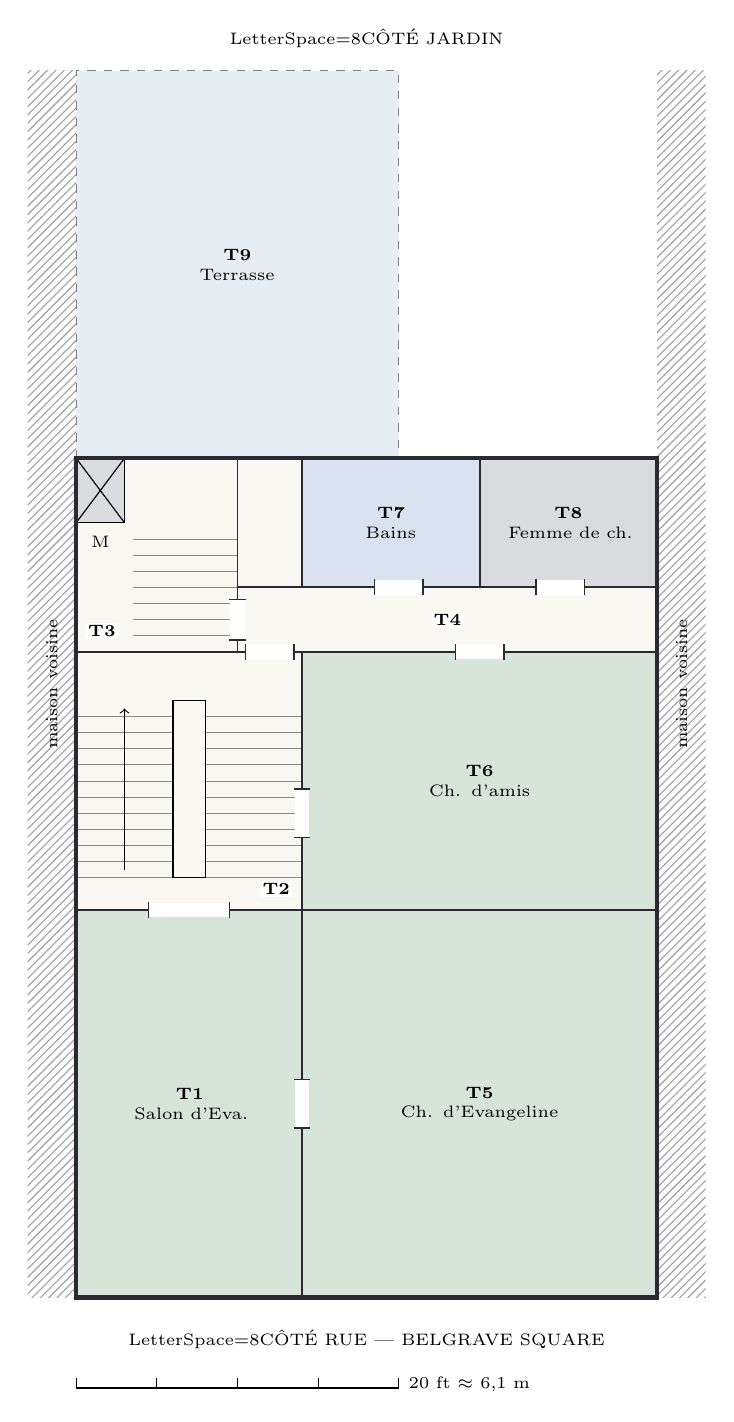
\begin{tikzpicture}[x=0.205cm,y=0.205cm]
\fill[pattern=north east lines, pattern color=wallc!45] (-3,0) rectangle (0,76);
\fill[pattern=north east lines, pattern color=wallc!45] (36,0) rectangle (39,76);
\node[tiny,rotate=90] at (-1.5,38) {maison voisine};
\node[tiny,rotate=90] at (37.5,38) {maison voisine};
\node[tiny] at (18,-2.6) {\caps{côté rue — Belgrave Square}};
\node[tiny] at (18,78) {\caps{côté jardin}};
\fill[fam] (0,0) rectangle (14,24);
\fill[cir] (0,24) rectangle (14,40);
\fill[cir] (0,40) rectangle (10,52);
\fill[cir] (10,40) rectangle (36,44);
\fill[cir] (10,44) rectangle (14,52);
\fill[fam] (14,0) rectangle (36,24);
\fill[fam] (14,24) rectangle (36,40);
\fill[san] (14,44) rectangle (25,52);
\fill[srv] (25,44) rectangle (36,52);
\fill[ext] (0,52) rectangle (20,76);
\fill[cir] (0,24) rectangle (14,40);
\draw[tread] (0,26) -- (6.0,26);
\draw[tread] (8.0,26) -- (14,26);
\draw[tread] (0,27) -- (6.0,27);
\draw[tread] (8.0,27) -- (14,27);
\draw[tread] (0,28) -- (6.0,28);
\draw[tread] (8.0,28) -- (14,28);
\draw[tread] (0,29) -- (6.0,29);
\draw[tread] (8.0,29) -- (14,29);
\draw[tread] (0,30) -- (6.0,30);
\draw[tread] (8.0,30) -- (14,30);
\draw[tread] (0,31) -- (6.0,31);
\draw[tread] (8.0,31) -- (14,31);
\draw[tread] (0,32) -- (6.0,32);
\draw[tread] (8.0,32) -- (14,32);
\draw[tread] (0,33) -- (6.0,33);
\draw[tread] (8.0,33) -- (14,33);
\draw[tread] (0,34) -- (6.0,34);
\draw[tread] (8.0,34) -- (14,34);
\draw[tread] (0,35) -- (6.0,35);
\draw[tread] (8.0,35) -- (14,35);
\draw[tread] (0,36) -- (6.0,36);
\draw[tread] (8.0,36) -- (14,36);
\draw[thin] (6.0,26) rectangle (8.0,37);
\draw[->,thin] (3.0,26.5) -- (3.0,36.5);
\fill[cir] (0,40) rectangle (10,52);
\draw[tread] (3.5,41) -- (10,41);
\draw[tread] (3.5,42) -- (10,42);
\draw[tread] (3.5,43) -- (10,43);
\draw[tread] (3.5,44) -- (10,44);
\draw[tread] (3.5,45) -- (10,45);
\draw[tread] (3.5,46) -- (10,46);
\draw[tread] (3.5,47) -- (10,47);
\fill[srv] (0,48) rectangle (3,52); \draw[thin] (0,48) rectangle (3,52);
\draw[thin] (0,48) -- (3,52) (0,52) -- (3,48);
\node[tiny] at (1.5,46.8) {M};
\draw[wall] (0,0) rectangle (14,24);
\draw[wall] (0,24) rectangle (14,40);
\draw[wall] (0,40) rectangle (10,52);
\draw[wall] (10,40) rectangle (36,44);
\draw[wall] (10,44) rectangle (14,52);
\draw[wall] (14,0) rectangle (36,24);
\draw[wall] (14,24) rectangle (36,40);
\draw[wall] (14,44) rectangle (25,52);
\draw[wall] (25,44) rectangle (36,52);
\draw[extwall] (0,52) rectangle (20,76);
\draw[outer] (0,0) rectangle (36,52);
\fill[white] (4.5,23.55) rectangle (9.5,24.45);
\draw[jamb] (4.5,23.5) -- (4.5,24.5) (9.5,23.5) -- (9.5,24.5);
\fill[white] (13.55,10.5) rectangle (14.45,13.5);
\draw[jamb] (13.5,10.5) -- (14.5,10.5) (13.5,13.5) -- (14.5,13.5);
\fill[white] (13.55,28.5) rectangle (14.45,31.5);
\draw[jamb] (13.5,28.5) -- (14.5,28.5) (13.5,31.5) -- (14.5,31.5);
\fill[white] (10.5,39.55) rectangle (13.5,40.45);
\draw[jamb] (10.5,39.5) -- (10.5,40.5) (13.5,39.5) -- (13.5,40.5);
\fill[white] (23.5,39.55) rectangle (26.5,40.45);
\draw[jamb] (23.5,39.5) -- (23.5,40.5) (26.5,39.5) -- (26.5,40.5);
\fill[white] (18.5,43.55) rectangle (21.5,44.45);
\draw[jamb] (18.5,43.5) -- (18.5,44.5) (21.5,43.5) -- (21.5,44.5);
\fill[white] (28.5,43.55) rectangle (31.5,44.45);
\draw[jamb] (28.5,43.5) -- (28.5,44.5) (31.5,43.5) -- (31.5,44.5);
\fill[white] (9.55,40.75) rectangle (10.45,43.25);
\draw[jamb] (9.5,40.75) -- (10.5,40.75) (9.5,43.25) -- (10.5,43.25);
\node[lab, text width=2.72cm] at (7,12) {\textbf{T1}\\ Salon d'Eva.};
\node[lab, text width=4.36cm] at (25,12) {\textbf{T5}\\ Ch. d'Evangeline};
\node[lab, text width=4.36cm] at (25,32) {\textbf{T6}\\ Ch. d'amis};
\node[lab, text width=2.10cm] at (19.5,48) {\textbf{T7}\\ Bains};
\node[lab, text width=2.10cm] at (30.5,48) {\textbf{T8}\\ Femme de ch.};
\node[lab, text width=3.95cm] at (10,64) {\textbf{T9}\\ Terrasse};
\node[numtag] at (12.4,25.3) {T2};
\node[numtag] at (1.6,41.3) {T3};
\node[numtag] at (23,42) {T4};
\begin{scope}[shift={(0,-5.6)}]
\draw[thin] (0,0) -- (20,0); \foreach \i in {0,5,...,20} \draw[thin] (\i,0) -- (\i,0.6);
\node[tiny,anchor=west] at (20.5,0.2) {20 ft $\approx$ 6,1 m};
\end{scope}
\end{tikzpicture}
\end{minipage}\hfill\begin{minipage}[t]{8.95cm}\vspace{0pt}\fontsize{8.4}{10.2}\selectfont
\begin{descr}
\item[\textbf{T1}] \textbf{Salon d'Evangeline}. Son petit salon personnel : piano droit, partitions annotées, fleurs séchées, portrait de sa mère. Elle y répète.
\item[\textbf{T5}] \textbf{Chambre d'Evangeline}. Chambre claire sur le square, papier peint fleuri. Elle y cache le médaillon au portrait de Théodore Eristoff.
\item[\textbf{T6}] \textbf{Chambre d'amis}. Seconde chambre d'invité, plus simple.
\item[\textbf{T7}] \textbf{Salle de bain des dames}. Kerr prévoit à cet étage « a second Bath-room (for ladies) ».
\item[\textbf{T8}] \textbf{Chambre de la femme de chambre}. La femme de chambre de Lady Whitmore, plus considérée que les autres servantes, loge près de sa maîtresse plutôt que sous les toits.
\item[\textbf{T9}] \textbf{Terrasse (toit de l'aile)}. Toit plat couvert de plomb.
\end{descr}
\end{minipage}
\newpage
\niveau{Combles — les chambres de domestiques}
{\small\textit{Hauteur : env. 8 ft sous le brisis du toit mansardé (2,45 m).}}\par
{\small Sous le toit, on n'accède à ce niveau que par l'escalier de service. Il fait froid l'hiver et étouffant l'été. Les servantes y logent à deux par chambre.}\par\vspace{4pt}
\noindent\begin{minipage}[t]{8.75cm}\vspace{0pt}
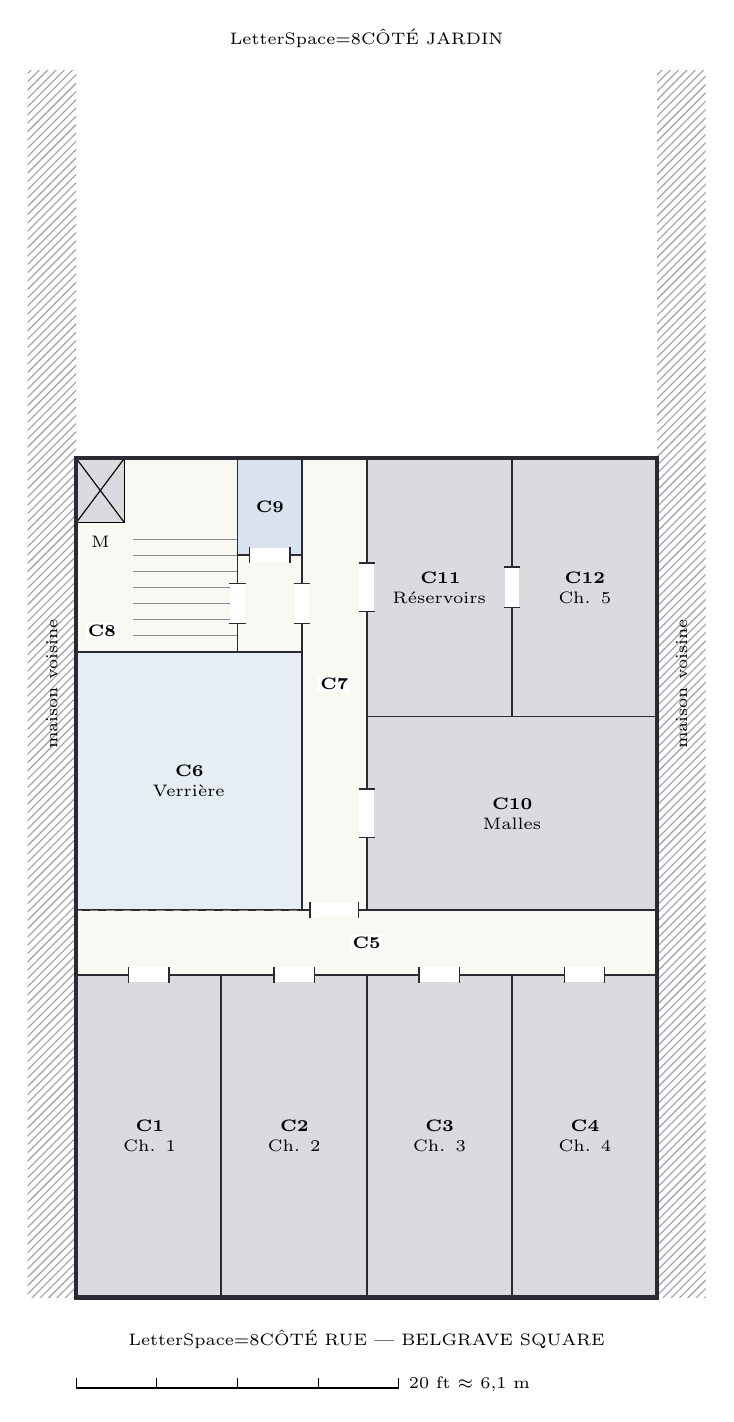
\begin{tikzpicture}[x=0.205cm,y=0.205cm]
\fill[pattern=north east lines, pattern color=wallc!45] (-3,0) rectangle (0,76);
\fill[pattern=north east lines, pattern color=wallc!45] (36,0) rectangle (39,76);
\node[tiny,rotate=90] at (-1.5,38) {maison voisine};
\node[tiny,rotate=90] at (37.5,38) {maison voisine};
\node[tiny] at (18,-2.6) {\caps{côté rue — Belgrave Square}};
\node[tiny] at (18,78) {\caps{côté jardin}};
\fill[srv] (0,0) rectangle (9,20);
\fill[srv] (9,0) rectangle (18,20);
\fill[srv] (18,0) rectangle (27,20);
\fill[srv] (27,0) rectangle (36,20);
\fill[cir] (0,20) rectangle (36,24);
\fill[ext] (0,24) rectangle (14,40);
\fill[cir] (14,24) rectangle (18,52);
\fill[cir] (10,40) rectangle (14,46);
\fill[cir] (0,40) rectangle (10,52);
\fill[san] (10,46) rectangle (14,52);
\fill[srv] (18,24) rectangle (36,36);
\fill[srv] (18,36) rectangle (27,52);
\fill[srv] (27,36) rectangle (36,52);
\fill[cir] (0,40) rectangle (10,52);
\draw[tread] (3.5,41) -- (10,41);
\draw[tread] (3.5,42) -- (10,42);
\draw[tread] (3.5,43) -- (10,43);
\draw[tread] (3.5,44) -- (10,44);
\draw[tread] (3.5,45) -- (10,45);
\draw[tread] (3.5,46) -- (10,46);
\draw[tread] (3.5,47) -- (10,47);
\fill[srv] (0,48) rectangle (3,52); \draw[thin] (0,48) rectangle (3,52);
\draw[thin] (0,48) -- (3,52) (0,52) -- (3,48);
\node[tiny] at (1.5,46.8) {M};
\draw[wall] (0,0) rectangle (9,20);
\draw[wall] (9,0) rectangle (18,20);
\draw[wall] (18,0) rectangle (27,20);
\draw[wall] (27,0) rectangle (36,20);
\draw[wall] (0,20) rectangle (36,24);
\draw[extwall] (0,24) rectangle (14,40);
\draw[wall] (14,24) rectangle (18,52);
\draw[wall] (10,40) rectangle (14,46);
\draw[wall] (0,40) rectangle (10,52);
\draw[wall] (10,46) rectangle (14,52);
\draw[wall] (18,24) rectangle (36,36);
\draw[wall] (18,36) rectangle (27,52);
\draw[wall] (27,36) rectangle (36,52);
\draw[outer] (0,0) rectangle (36,52);
\fill[white] (3.25,19.55) rectangle (5.75,20.45);
\draw[jamb] (3.25,19.5) -- (3.25,20.5) (5.75,19.5) -- (5.75,20.5);
\fill[white] (12.25,19.55) rectangle (14.75,20.45);
\draw[jamb] (12.25,19.5) -- (12.25,20.5) (14.75,19.5) -- (14.75,20.5);
\fill[white] (21.25,19.55) rectangle (23.75,20.45);
\draw[jamb] (21.25,19.5) -- (21.25,20.5) (23.75,19.5) -- (23.75,20.5);
\fill[white] (30.25,19.55) rectangle (32.75,20.45);
\draw[jamb] (30.25,19.5) -- (30.25,20.5) (32.75,19.5) -- (32.75,20.5);
\fill[white] (14.5,23.55) rectangle (17.5,24.45);
\draw[jamb] (14.5,23.5) -- (14.5,24.5) (17.5,23.5) -- (17.5,24.5);
\fill[white] (17.55,28.5) rectangle (18.45,31.5);
\draw[jamb] (17.5,28.5) -- (18.5,28.5) (17.5,31.5) -- (18.5,31.5);
\fill[white] (17.55,42.5) rectangle (18.45,45.5);
\draw[jamb] (17.5,42.5) -- (18.5,42.5) (17.5,45.5) -- (18.5,45.5);
\fill[white] (26.55,42.75) rectangle (27.45,45.25);
\draw[jamb] (26.5,42.75) -- (27.5,42.75) (26.5,45.25) -- (27.5,45.25);
\fill[white] (9.55,41.75) rectangle (10.45,44.25);
\draw[jamb] (9.5,41.75) -- (10.5,41.75) (9.5,44.25) -- (10.5,44.25);
\fill[white] (13.55,41.75) rectangle (14.45,44.25);
\draw[jamb] (13.5,41.75) -- (14.5,41.75) (13.5,44.25) -- (14.5,44.25);
\fill[white] (10.75,45.55) rectangle (13.25,46.45);
\draw[jamb] (10.75,45.5) -- (10.75,46.5) (13.25,45.5) -- (13.25,46.5);
\node[lab, text width=1.70cm] at (4.5,10) {\textbf{C1}\\ Ch. 1};
\node[lab, text width=1.70cm] at (13.5,10) {\textbf{C2}\\ Ch. 2};
\node[lab, text width=1.70cm] at (22.5,10) {\textbf{C3}\\ Ch. 3};
\node[lab, text width=1.70cm] at (31.5,10) {\textbf{C4}\\ Ch. 4};
\node[lab, text width=2.72cm] at (7,32) {\textbf{C6}\\ Verrière};
\node[lab] at (12,49) {\textbf{C9}};
\node[lab, text width=3.54cm] at (27,30) {\textbf{C10}\\ Malles};
\node[lab, text width=1.70cm] at (22.5,44) {\textbf{C11}\\ Réservoirs};
\node[lab, text width=1.70cm] at (31.5,44) {\textbf{C12}\\ Ch. 5};
\node[numtag] at (18,22) {C5};
\node[numtag] at (16,38) {C7};
\node[numtag] at (1.6,41.3) {C8};
\begin{scope}[shift={(0,-5.6)}]
\draw[thin] (0,0) -- (20,0); \foreach \i in {0,5,...,20} \draw[thin] (\i,0) -- (\i,0.6);
\node[tiny,anchor=west] at (20.5,0.2) {20 ft $\approx$ 6,1 m};
\end{scope}
\end{tikzpicture}
\end{minipage}\hfill\begin{minipage}[t]{8.95cm}\vspace{0pt}\fontsize{8.4}{10.2}\selectfont
\begin{descr}
\item[\textbf{C1}] \textbf{Chambre de domestiques 1}. Lit de fer, commode, cuvette et broc, crochets aux murs. Lucarne sur le square.
\item[\textbf{C2}] \textbf{Chambre de domestiques 2}. Idem.
\item[\textbf{C3}] \textbf{Chambre de domestiques 3}. Idem.
\item[\textbf{C4}] \textbf{Chambre de domestiques 4}. Idem.
\item[\textbf{C6}] \textbf{Verrière du grand escalier}. Lanterneau vitré au-dessus de la cage du grand escalier.
\item[\textbf{C8}] \textbf{Escalier de service}. Arrivée de l'escalier de service, seul accès aux combles.
\item[\textbf{C10}] \textbf{Chambre aux malles}. Malles de voyage, cartons à chapeaux, meubles hors d'usage. Kerr : « Luggage and Lumber-rooms ».
\item[\textbf{C11}] \textbf{Réservoirs d'eau}. Citernes alimentées par la compagnie des eaux ; elles donnent la pression à l'eau froide des étages.
\item[\textbf{C12}] \textbf{Chambre de domestiques 5}. Idem.
\end{descr}
\end{minipage}
\newpage
\niveau{Sources et repères}
\begin{itemize}[leftmargin=1.2em,itemsep=3pt]
\item Robert Kerr, \emph{The Gentleman's House}, 3\textsuperscript{e} éd., 1871, pl.~XLII, « Design for London Houses » : répartition des pièces par étage, monte-charge dans l'escalier de service, écuries sur la ruelle arrière. Texte reproduit sur \emph{Victorian London} (victorianlondon.org, « A London Town House »).
\item Belgrave Square : terraces dessinés par George Basevi pour Lord Grosvenor dans les années 1820, maisons en stuc blanc, occupées pour la plupart vers 1840 (Wikipédia, « Belgrave Square »).
\item Équipements : salles de bain fixes à eau chaude et froide dans les grandes maisons après 1870 ; cuvette de WC tout en céramique présentée en 1884 ; manchon à incandescence Welsbach à partir de 1885 ; électricité dans une partie de Kensington dès 1887, mais encore très rare (UWE, « Victorian \& Edwardian Services (Houses) 1850--1914 »).
\item Références de décor possibles : 18 Stafford Terrace (Kensington), maison d'Edward Linley Sambourne, conservée avec son intérieur des années 1870--1900.
\end{itemize}

\textbf{Choix ouverts.} Le square exact, la décoration de chaque pièce, l'éclairage (gaz seul, ou électricité dans les salons, ce qui serait un luxe rare), la position précise des horloges et le nombre de domestiques présents ce soir. Personnel supposé : majordome, deux valets de pied, cuisinière, fille de cuisine, fille d'arrière-cuisine, deux femmes de chambre, la femme de chambre de Lady Whitmore, un cocher et un palefrenier aux écuries. Mrs.~Hartwell, l'intendante, est au manoir avec Lord Whitmore.
\end{document}
